\documentclass[11pt]{article}

\usepackage[margin=1.15in]{geometry}
\usepackage{amsmath}
\usepackage{amssymb}
\usepackage{graphicx}
\usepackage{xcolor}
% keeps a paragraph heading with the list that follows it
\usepackage{needspace}
\usepackage[hidelinks]{hyperref}

% One symbol per object.  The aperture mass and its moments.
\newcommand{\Map}{M_{\rm ap}}
\newcommand{\Mx}{M_{\times}}
% The compensated filter in real and Fourier space.
\newcommand{\Ufil}{U_R}
\newcommand{\Qfil}{Q_R}
\newcommand{\Uhat}{\widehat{U}}
% Vectors on the flat sky and in Fourier space.
\newcommand{\btheta}{\boldsymbol{\theta}}
\newcommand{\bell}{\boldsymbol{\ell}}
\newcommand{\bk}{\boldsymbol{k}}
% An underscore after which a long code name may break.
\newcommand{\us}{\_\allowbreak}

\title{The third-order aperture-mass statistic}
\date{November 2026}
\author{}

\emergencystretch=3em
% let the figures share a page with text (no figure-only pages)
\renewcommand{\topfraction}{0.9}
\renewcommand{\bottomfraction}{0.8}
\renewcommand{\textfraction}{0.07}
\renewcommand{\floatpagefraction}{0.85}
\setcounter{topnumber}{3}
\setcounter{totalnumber}{4}

\begin{document}

\begin{center}
  {\LARGE The third-order aperture-mass statistic\par}
  \vspace{0.4em}
  {\large From galaxy shapes to the $\langle\Map^3\rangle$ rows of the
    joint shear likelihood, built up from first principles\par}
  \vspace{0.6em}
  {\large November 2026\par}
\end{center}
\vspace{0.5em}

\tableofcontents
\vspace{1em}

\section{Summary}
\label{sec:summary}

\paragraph{The question.}
The DES Y3 joint shear likelihood of this project scores a data vector
with two parts: the shear two-point correlations $\xi_\pm$, and $80$
entries called $\langle\Map^3\rangle$, the third moment of the
aperture mass (the measured counts are checked in
Section~\ref{sec:fiducial}).  What is the aperture mass?  Why is its
third moment a good carrier of three-point information?  And what,
exactly, does the likelihood compute when it predicts those $80$
numbers?  This note builds the answer from the ground up, assuming
only calculus, linear algebra, complex numbers and basic Fourier
transforms; everything else -- correlation functions, ensemble
averages, the bispectrum, spin-2 fields, Bessel functions -- is
introduced where it first appears.

\paragraph{The answer, in one list.}
\begin{enumerate}
  \item Gravitational lensing turns the matter between us and distant
    galaxies into two observable fields on the sky: the convergence
    $\kappa$ (a magnification) and the shear $\gamma$ (a stretching of
    galaxy images).  Both are random fields, described by their
    statistical moments (Sections~\ref{sec:fields}
    and~\ref{sec:lensing}).
  \item The aperture mass $\Map(R)$ is the convergence averaged inside
    a circle of radius $R$ with a weight that integrates to zero -- a
    compensated filter.  That one property makes it blind to any
    constant mass sheet, measurable from galaxy shapes alone, and a
    clean separator of the lensing-like E~pattern from the B~pattern
    that lensing does not produce (Section~\ref{sec:aperture}).
  \item Its variance $\langle\Map^2\rangle$ reads the convergence
    power spectrum through a narrow window of multipoles around
    $\ell \approx \sqrt{2}/R$; its third moment
    $\langle\Map^3\rangle$ reads the convergence bispectrum, the
    lowest-order statistic that is zero for a Gaussian field
    (Sections~\ref{sec:map2} and~\ref{sec:map3}).
  \item In practice nobody integrates filters over a map full of
    masks and holes.  The measurement and the likelihood both take a
    detour through the shear three-point correlation function: its
    four natural components $\Gamma_0,\ldots,\Gamma_3$ on triangles,
    integrated with known kernels, reproduce
    $\langle\Map^3\rangle$ (Section~\ref{sec:threepcf}).
  \item Integrating only over the finitely many measured triangle bins
    defines a slightly different estimator than the infinite filter
    integral.  That difference is why the project refuses to produce
    an analytic Map3 covariance: the compiled covariance describes the
    full-filter estimator, not the finite one
    (Section~\ref{sec:finite}).
  \item The DES Y3 measurement and the likelihood settings -- the side
    bins, the scale cut, the four filter radii, the source-bin
    triplets -- are listed with the keys that control them
    (Section~\ref{sec:likelihood}).
  \item Galaxy shapes also align with the local tidal field, without
    any lensing.  The tidal alignment and tidal torquing (TATT) model
    of Gomes et al.~\cite{GomesTATT} predicts how that contaminates
    $\langle\Map^3\rangle$; Section~\ref{sec:ia} rebuilds that theory
    from elementary probability and calculus and connects it to the
    operator split the project code computes.
\end{enumerate}

\paragraph{The setup.}
The data are the DES (Dark Energy Survey) Year 3 weak-lensing
products bundled with the project: $400$ two-point entries
($200$ $\xi_+$ and $200$ $\xi_-$) and $80$ aperture entries, with
four tomographic source bins (galaxies sorted into four groups by
estimated redshift).  The likelihood is
\texttt{des\us 3pcf.joint\us shear}; its numerical settings live in
\texttt{likelihood/joint\us shear.yaml}, and the fiducial evaluation
point is the \texttt{override} block of
\texttt{EXAMPLE\us EVALUATE1.yaml} (Section~\ref{sec:fiducial}).  The
companion notebook \texttt{aperture\us mass\us statistic.ipynb},
beside this note, recomputes every number this note quotes and
rebuilds every figure; its toy models (a simulated convergence map, a
white-noise spectrum) run in seconds, and its real predictions go
through the project's own wrappers,
\texttt{interface/cosmolike\us des\us 3pcf\us notebook\us
wrappers.py}.

\paragraph{How to read this note.}
The note is long because it assumes little.  A first pass can take
the short route:
\begin{enumerate}
  \item Section~\ref{sec:aperture} up to
    Eq.~\eqref{eq:uhat}: what the aperture mass is, why the
    compensated filter kills a constant sheet, and which angular
    scales $\Map(R)$ actually probes.
  \item The opening of Section~\ref{sec:map3}: the third moment as a
    triple Fourier integral over the bispectrum,
    Eq.~\eqref{eq:map3full}.
  \item Section~\ref{sec:threepcf} up to Eq.~\eqref{eq:map3sas}: how
    the same number is obtained from measured triangles, which is
    what the likelihood does.
  \item The opening of Section~\ref{sec:finite}: why the finite
    triangle sum is a different estimator, and the covariance
    consequence.
\end{enumerate}
A reader who wants the foundations -- what a correlation function is,
why a Gaussian field has no third moment, where the $e^{2i\beta}$
phase of the shear comes from -- starts instead at
Section~\ref{sec:fields} and reads straight through.  The
intrinsic-alignment theory of Section~\ref{sec:ia} stands on its own
and can be read last; it depends only on
Sections~\ref{sec:fields}--\ref{sec:map3}.

\section{Fiducial model and parameter values}
\label{sec:fiducial}

This section freezes the point at which every prediction of this note
and its companion notebook is evaluated, so the note does not depend
on files that may drift.

\paragraph{The cosmology and nuisance parameters.}
The fiducial point is the \texttt{override} block -- the entries that
pin the evaluation point -- of \texttt{EXAMPLE\us EVALUATE1.yaml}
(Table~\ref{tab:fid}).  The model is flat $w$CDM with $w = -1$:
$\Omega_{\rm m}$ is the matter density today in units of the critical
density, $\Omega_{\rm b}$ the baryon part of it, $h$ the Hubble
constant in units of $100$~km/s/Mpc, $n_{\rm s}$ the tilt of the
primordial power spectrum, and $\sigma_8$ the rms linear density
contrast in spheres of $8\,h^{-1}$Mpc, the amplitude the project
samples directly.  The intrinsic-alignment model of this yaml is NLA
(defined in Section~\ref{sec:ia}): the linear amplitude $A_1$ and its
redshift slope $\eta_1$ are nonzero, while the quadratic TATT
parameters $A_2$, $\eta_2$ and $b_{\rm TA}$ are fixed to zero.  The
$m_i$ are the multiplicative shear calibrations of the four source
bins ($\gamma \to (1+m_i)\gamma$), and the $\Delta z_i$ shift each
source redshift distribution.

\begin{table}[tbp]
  \centering
  \small
  \begin{tabular}{lll}
    \hline
    parameter & meaning & fiducial \\
    \hline
    $\Omega_{\rm m}$ & matter density today & $0.289$ \\
    $\Omega_{\rm b}$ & baryon density today & $0.0463$ \\
    $h$ & Hubble constant / ($100$ km/s/Mpc) & $0.722$ \\
    $n_{\rm s}$ & scalar spectral index & $0.959$ \\
    $\sigma_8$ & amplitude of linear fluctuations & $0.7865548$ \\
    $A_1$ & linear (tidal-alignment) IA amplitude & $-0.33$ \\
    $\eta_1$ & its redshift slope & $2.81$ \\
    $A_2,\ \eta_2,\ b_{\rm TA}$ & quadratic TATT parameters & $0$ \\
    $m_1,\ldots,m_4$ & shear calibrations & $-0.0063$, $-0.0198$, $-0.0241$, $-0.0369$ \\
    $\Delta z_1,\ldots,\Delta z_4$ & source photo-z shifts & $0$ \\
    $w_0,\ w_a$ & dark-energy equation of state & $-1$, $0$ (fixed) \\
    $\sum m_\nu$ & neutrino mass sum [eV] & $0.06$ (fixed) \\
    \hline
  \end{tabular}
  \caption{The fiducial point: the evaluate \texttt{override} of
    \texttt{EXAMPLE\us EVALUATE1.yaml}, plus the parameters that yaml
    fixes.  $\sigma_8$ is quoted to seven digits here; the yaml
    carries the full value.  The companion notebook prints every
    value from the yaml (its Section~4).}
  \label{tab:fid}
\end{table}

\paragraph{The TATT point of the intrinsic-alignment section.}
Section~\ref{sec:ia} needs a point where the quadratic alignment
terms are switched on.  It uses the \texttt{override} of
\texttt{EXAMPLE\us EVALUATE2.yaml}: the same cosmology, calibrations
and shifts as Table~\ref{tab:fid}, with
\begin{equation}
  A_2 = 0.65, \qquad \eta_2 = 1.69, \qquad b_{\rm TA} = 0.91 .
  \label{eq:tattpoint}
\end{equation}

\paragraph{The data layout.}
At this point the likelihood's data vector has $480$ rows: $200$
$\xi_+$, $200$ $\xi_-$ and $80$ aperture rows.  The aperture rows are
the $20$ source-bin triplets (all unordered triples from four bins,
Section~\ref{sec:map3}) times the four equal filter radii
\begin{equation}
  R \;=\; 7,\ 14,\ 25,\ 40 \ \text{arcmin},
  \label{eq:radii}
\end{equation}
read from the measurement file.  The three-point correlations behind
them live on side bins defined by the likelihood keys
(Section~\ref{sec:likelihood}): $20$ logarithmic bins from $0.5$ to
$80$ arcmin, of which the scale cut keeps the $9$ whose lower edge is
at least $8$ arcmin.  Every one of these counts is recomputed and
printed by the companion notebook (its Section~5).

\paragraph{Theory inputs.}
CAMB supplies distances, growth and the matter power spectrum;
BiHalofit~\cite{BiHalofit}, a fitting formula calibrated on N-body
simulations, supplies the nonlinear matter bispectrum.  Both run as
Cobaya theory blocks of the example yaml; the likelihood never runs a
private copy of either.

\section{Random fields on the sky}
\label{sec:fields}

This section defines the statistical language: ensemble averages,
correlation functions, the power spectrum, connected moments and the
bispectrum.  Everything later is an application of these definitions.

\subsection{Ensemble averages and correlation functions}
\label{sec:ensemble}

\paragraph{A random field.}
A field assigns a number to every position; on a small patch of sky we
use flat coordinates $\btheta = (\theta_x, \theta_y)$ and write, for
example, $\kappa(\btheta)$.  A \emph{random} field is one whose values
we model as drawn from a probability distribution: cosmology does not
predict the value of $\kappa$ toward one particular galaxy, it
predicts the statistics of $\kappa$ over many realizations of the
initial conditions of the Universe.  The angle bracket
$\langle\cdot\rangle$ denotes this \emph{ensemble average}: the mean
over all realizations, with each weighted by its probability.  In
practice we observe one sky, and averaging over many well-separated
patches of it stands in for the ensemble average.

\paragraph{Homogeneity and isotropy.}
Two assumptions make the statistics manageable.  \emph{Statistical
homogeneity}: the distribution does not single out a position, so any
average of field values depends only on the separations between the
points, not on where the configuration sits.  \emph{Statistical
isotropy}: it does not single out a direction, so the average is also
unchanged when the whole configuration is rotated.  For the two-point
function of a zero-mean field ($\langle\kappa\rangle = 0$) these
assumptions leave a function of one number, the separation
$\theta = |\btheta_1 - \btheta_2|$:
\begin{equation}
  \xi(\theta) \;=\;
  \bigl\langle \kappa(\btheta_1)\,\kappa(\btheta_2) \bigr\rangle .
  \label{eq:xidef}
\end{equation}
$\xi(\theta) > 0$ means that where the field is high, it tends to be
high a distance $\theta$ away as well.

\paragraph{A two-variable toy.}
Correlation is best seen with two plain random variables before any
field appears.  Let $x$ and $y$ be zero-mean Gaussian variables with
\begin{equation}
  \langle x^2 \rangle = 1, \qquad
  \langle y^2 \rangle = 1, \qquad
  \langle x y \rangle = 0.8 .
  \label{eq:toyxy}
\end{equation}
Draw many pairs and scatter them: the cloud is a tilted ellipse, and
knowing $x$ shrinks the spread of $y$ from $1$ to
$\sqrt{1 - 0.8^2} = 0.6$.  A field's $\xi(\theta)$ is exactly this
$\langle xy\rangle$, with $x = \kappa$ at one point and $y = \kappa$
at a point a distance $\theta$ away.

\subsection{Fourier modes and the power spectrum}
\label{sec:power}

\paragraph{The flat-sky Fourier transform.}
On a flat patch, decompose the field into plane waves,
\begin{equation}
  \kappa(\btheta) \;=\;
  \int \frac{d^2\ell}{(2\pi)^2}\,
  \tilde\kappa(\bell)\, e^{\,i \bell\cdot\btheta},
  \qquad
  \tilde\kappa(\bell) \;=\;
  \int d^2\theta\, \kappa(\btheta)\, e^{-i \bell\cdot\btheta}.
  \label{eq:fourier}
\end{equation}
The vector $\bell$ is the angular frequency: the wave
$e^{i\bell\cdot\btheta}$ repeats after an angle $2\pi/\ell$ along the
direction of $\bell$, so a larger multipole $\ell = |\bell|$ means a
finer angular pattern.  One arcminute corresponds to
$\ell \approx 2\pi/(1' \text{ in radians}) \approx 2\times 10^4$.

\paragraph{The power spectrum.}
For a homogeneous field, different Fourier modes are uncorrelated,
and the two-point statistics collapse to one function of $\ell$:
\begin{equation}
  \bigl\langle \tilde\kappa(\bell_1)\,\tilde\kappa(\bell_2)
  \bigr\rangle
  \;=\; (2\pi)^2\, \delta_{\rm D}(\bell_1 + \bell_2)\,
  P_\kappa(\ell_1).
  \label{eq:powerdef}
\end{equation}
Here $\delta_{\rm D}$ is the Dirac delta, the sharp spike defined by
$\int d^2\ell\, \delta_{\rm D}(\bell) f(\bell) = f(0)$.  Its presence
is the Fourier-space face of homogeneity: a correlation between modes
with $\bell_1 + \bell_2 \neq 0$ would, transformed back, make
$\xi$ depend on absolute position, which homogeneity forbids.  The
power spectrum $P_\kappa(\ell)$ is the variance carried by modes of
angular frequency $\ell$; it and $\xi(\theta)$ contain the same
information, as a transform pair.

\subsection{Third moments, connected parts and the bispectrum}
\label{sec:bispectrum}

\paragraph{Connected moments, with two variables.}
A third moment can be large merely because the variables have large
means or variances.  The \emph{connected} moment is what remains
after subtracting everything that lower moments already predict.  For
one zero-mean variable $x$ the connected third moment is simply
$\langle x^3\rangle$, the skewness numerator: the lower moments
$\langle x\rangle = 0$ and $\langle x^2\rangle$ predict no third
moment at all, because a distribution can be symmetric
($x \to -x$) with any variance, and symmetry forces
$\langle x^3\rangle = 0$.  With a mean the subtraction is explicit:
\begin{equation}
  \langle x y \rangle_{\rm c}
  \;=\; \langle x y \rangle - \langle x\rangle\langle y \rangle ,
  \label{eq:connected2}
\end{equation}
and for three zero-mean variables
\begin{equation}
  \langle x y z \rangle_{\rm c} \;=\; \langle x y z \rangle ,
  \label{eq:connected3}
\end{equation}
because every product of lower moments
($\langle x\rangle\langle yz\rangle$ and its relabelings,
$\langle x\rangle\langle y\rangle\langle z\rangle$) contains at least
one vanishing mean.  All cosmological fields below are zero-mean, so
their third moments are already connected.

\paragraph{A Gaussian field has no third moment.}
A zero-mean Gaussian variable has the symmetric density
$p(x) \propto e^{-x^2/2\sigma^2}$, so $\langle x^3\rangle = 0$: the
integrand $x^3 p(x)$ is odd.  The same holds jointly: for zero-mean
Gaussian variables, every odd moment vanishes, because the joint
density is unchanged under flipping the sign of all variables at
once, while the product $xyz$ flips sign.  A Gaussian \emph{field} is
one whose values at any set of points are jointly Gaussian; its
three-point function therefore vanishes identically.  This is the key
fact of this note: \textbf{any measured third moment is a direct
detection of non-Gaussianity}.  The primordial fluctuations were very
close to Gaussian; gravity made them non-Gaussian, because collapse
is not symmetric -- overdense regions contract and deepen without
bound, while underdense regions can at most empty out to
$\delta = -1$.  The companion notebook makes this concrete: the
skewness of a simulated Gaussian convergence map is consistent with
zero, within its sampling noise (its Section~3).

\paragraph{The bispectrum.}
The three-point analogue of Eq.~\eqref{eq:powerdef} defines the
bispectrum $B_\kappa$:
\begin{equation}
  \bigl\langle \tilde\kappa(\bell_1)\,\tilde\kappa(\bell_2)\,
  \tilde\kappa(\bell_3) \bigr\rangle
  \;=\; (2\pi)^2\, \delta_{\rm D}(\bell_1 + \bell_2 + \bell_3)\,
  B_\kappa(\ell_1, \ell_2, \ell_3).
  \label{eq:bispecdef}
\end{equation}
The delta again enforces homogeneity: only mode triples whose vectors
close into a triangle, $\bell_1 + \bell_2 + \bell_3 = 0$, correlate.
Isotropy then leaves a function of the triangle's shape and size
alone, written here through the three side lengths.  The same
definition in three dimensions, with wavevectors $\bk_i$ and a
$(2\pi)^3 \delta_{\rm D}^{(3)}$, defines the matter bispectrum
$B_{\rm m}(k_1,k_2,k_3;z)$, the quantity BiHalofit fits.

\paragraph{Why gravity makes a positive bispectrum.}
At the lowest order of perturbation theory, gravity corrects the
linear density field $\delta^{(1)}$ by a term quadratic in it,
$\delta \simeq \delta^{(1)} + \delta^{(2)}$ with
$\delta^{(2)} \sim (\delta^{(1)})^2$ schematically.  A third moment
then picks up its first nonzero contribution from one quadratic and
two linear factors,
\begin{equation}
  \bigl\langle \delta\,\delta\,\delta \bigr\rangle
  \;\simeq\;
  3\,\bigl\langle \delta^{(2)}\,\delta^{(1)}\,\delta^{(1)}
  \bigr\rangle ,
  \label{eq:treeidea}
\end{equation}
which contains \emph{four} linear (Gaussian) factors.  For zero-mean
jointly Gaussian variables the even moments follow the pair rule,
\begin{equation}
  \langle abcd \rangle \;=\;
  \langle ab\rangle\langle cd\rangle
  + \langle ac\rangle\langle bd\rangle
  + \langle ad\rangle\langle bc\rangle
  \label{eq:pairrule}
\end{equation}
(check it on one variable: $\langle x^4\rangle = 3\sigma^4$), so the
four-point average splits into products of two two-point functions
-- nonzero, and proportional to a product of two power spectra.
Written out in Fourier space this is the tree-level bispectrum
\begin{equation}
  B^{\rm tree}_{\delta}(\bk_1,\bk_2,\bk_3)
  \;=\;
  2 F_2(\bk_1,\bk_2) P_{\rm L}(k_1) P_{\rm L}(k_2)
  \;+\; \text{2 cyclic permutations},
  \label{eq:btree}
\end{equation}
where $P_{\rm L}$ is the linear matter power spectrum and
\begin{equation}
  F_2(\bk_1,\bk_2) \;=\; \frac{5}{7}
  + \frac{1}{2}\,\hat\bk_1\!\cdot\!\hat\bk_2
    \left(\frac{k_1}{k_2} + \frac{k_2}{k_1}\right)
  + \frac{2}{7}\,\bigl(\hat\bk_1\!\cdot\!\hat\bk_2\bigr)^2
  \label{eq:f2}
\end{equation}
is the second-order gravity kernel (hats denote unit vectors).  The
derivation of $F_2$ is standard perturbation theory and not repeated
here; what matters below is the \emph{structure} of
Eq.~\eqref{eq:btree} -- a quadratic kernel times two power spectra,
summed over which leg carries the kernel -- because the
intrinsic-alignment bispectra of Section~\ref{sec:ia} have exactly
the same structure with different kernels.  On nonlinear scales the
project replaces Eq.~\eqref{eq:btree} by the BiHalofit
fit~\cite{BiHalofit}, which is calibrated on simulations and reduces
to the tree level on large scales.

\section{Convergence and shear}
\label{sec:lensing}

\subsection{Lensing in two fields}
\label{sec:kappa}

\paragraph{The convergence.}
Light from a distant galaxy is deflected by the matter it passes.  To
first order the effect on the image is linear and has two parts: an
isotropic magnification, described by the \emph{convergence}
$\kappa$, and an area-preserving stretching, described by the
\emph{shear} $\gamma$.  The convergence toward direction $\btheta$
for source sample $a$ is a weighted integral of the matter density
contrast $\delta_{\rm m} = (\rho - \bar\rho)/\bar\rho$ along the line
of sight~\cite{GomesTATT}:
\begin{equation}
  \kappa_a(\btheta)
  \;=\; \frac{3\Omega_{\rm m} H_0^2}{2 c^2}
  \int_0^{\infty} d\chi\;
  q_a(\chi)\,
  \frac{\delta_{\rm m}\bigl(\chi\btheta, \chi;\, z(\chi)\bigr)}
       {a(\chi)} ,
  \label{eq:kappadef}
\end{equation}
where $\chi$ is the comoving distance, $a(\chi) = 1/(1+z)$ the scale
factor, and the \emph{lensing efficiency}
\begin{equation}
  q_a(\chi) \;=\;
  \int_\chi^{\infty} d\chi'\;
  p_a(\chi')\, \frac{\chi' - \chi}{\chi'}
  \label{eq:qdef}
\end{equation}
weights each foreground distance by how much of source sample $a$
(redshift distribution $p_a$, normalized to unit integral) lies
behind it and by the lens--source geometry: a lens halfway to the
source deflects most effectively.  The prefactor in
Eq.~\eqref{eq:kappadef} comes from Poisson's equation, which converts
a density contrast into a gravitational potential; its size,
$\Omega_{\rm m} H_0^2/c^2$, is why lensing measures the matter
density.  \emph{Tomography} means splitting the sources into samples
by estimated redshift -- four bins for DES Y3 -- so that each
$\kappa_a$ probes a different stretch of the line of sight.

\paragraph{The shear and its spin.}
The shear has two components: $\gamma_1$ stretches along the
coordinate axes, $\gamma_2$ along the diagonals.  They combine
naturally into one complex number
\begin{equation}
  \gamma \;=\; \gamma_1 + i\,\gamma_2 .
  \label{eq:gammacomplex}
\end{equation}
Rotate the coordinate axes by an angle $\varphi$ and the shear
components mix; written complexly, the transformation is a pure phase
\begin{equation}
  \gamma \;\longrightarrow\; \gamma\, e^{-2i\varphi} .
  \label{eq:spin2}
\end{equation}
The factor $2$ -- the statement that shear is a \emph{spin-2}
quantity -- has an elementary origin: a stretched image is an
ellipse, and an ellipse rotated by $180^\circ$ looks the same, so
the physical orientation angle lives on a half circle and appears in
formulas doubled.  (Compare a vector, spin~1, which needs a full
$360^\circ$ to return to itself, and transforms with
$e^{-i\varphi}$.)  Keeping track of this phase is most of the
bookkeeping of three-point shear statistics.

\paragraph{One potential behind both fields.}
Both $\kappa$ and $\gamma$ are second derivatives of a single lensing
potential $\psi(\btheta)$ (the weighted projection of the
gravitational potential along the line of sight):
\begin{equation}
  \kappa \;=\; \tfrac{1}{2}\bigl(\partial_1^2 + \partial_2^2\bigr)\psi,
  \qquad
  \gamma \;=\; \gamma_1 + i\gamma_2
  \;=\; \tfrac{1}{2}\bigl(\partial_1^2 - \partial_2^2\bigr)\psi
        + i\,\partial_1\partial_2\,\psi ,
  \label{eq:potential}
\end{equation}
with $\partial_j = \partial/\partial\theta_j$.  In Fourier space each
derivative $\partial_j$ becomes a factor $i\ell_j$, so with
$\bell = \ell(\cos\beta, \sin\beta)$,
\begin{equation}
  \tilde\kappa = -\tfrac{1}{2}\,\ell^2\,\tilde\psi,
  \qquad
  \tilde\gamma
  = -\tfrac{1}{2}\bigl(\ell_1^2 - \ell_2^2 + 2i\,\ell_1\ell_2\bigr)
    \tilde\psi
  = -\tfrac{1}{2}\,\ell^2 e^{2i\beta}\,\tilde\psi ,
  \label{eq:fourierpair}
\end{equation}
using
$\ell_1^2 - \ell_2^2 + 2i\ell_1\ell_2 = (\ell_1 + i\ell_2)^2 =
\ell^2 e^{2i\beta}$.  Dividing the two,
\begin{equation}
  \tilde\gamma(\bell) \;=\; \tilde\kappa(\bell)\, e^{2i\beta} ,
  \label{eq:gammakappa}
\end{equation}
where $\beta$ is the polar angle of $\bell$ (the direction of the
wave).  This one-line relation is the engine of the whole subject: every
statistic of the measurable $\gamma$ can be converted into a
statistic of the scalar $\kappa$, whose theory
(Eq.~\eqref{eq:kappadef}) is simple.  The companion notebook verifies
it constructively: it draws a Gaussian $\kappa$ map, manufactures the
shear field with Eq.~\eqref{eq:gammakappa} by FFT, and checks that
the two routes to the aperture mass defined below agree (its
Section~3).

\paragraph{E and B modes.}
Equation~\eqref{eq:gammakappa} produces a particular polarization
pattern: around an overdensity, images align tangentially, like rings
around a pond ripple.  This curl-free pattern is called the
\emph{E~mode}.  Its $45^\circ$-rotated partner -- a swirl -- is the
\emph{B~mode}, and no scalar lensing potential can produce it.  A
general shear field decomposes into both, replacing
Eq.~\eqref{eq:gammakappa} by
$\tilde\gamma = (\tilde\kappa_E + i \tilde\kappa_B) e^{2i\beta}$.
Measuring a B~mode therefore flags something other than weak lensing:
noise, systematics, or intrinsic alignments
(Section~\ref{sec:ia})~\cite{Crittenden}.  Locally, the shear at
separation $\btheta$ from a point is projected onto the
\emph{tangential} and \emph{cross} components
\begin{equation}
  \gamma_t + i\,\gamma_\times
  \;=\; -\,\gamma\, e^{-2i\phi_{\btheta}} ,
  \label{eq:tangential}
\end{equation}
with $\phi_{\btheta}$ the polar angle of the separation vector:
$\gamma_t > 0$ is a tangential stretch, and $\gamma_\times$ the
swirl component.

\section{The aperture mass}
\label{sec:aperture}

\subsection{A compensated filter}
\label{sec:filter}

\paragraph{The definition.}
The aperture mass at position $\btheta_0$ and radius $R$ is the
convergence averaged with a circular weight:
\begin{equation}
  \Map(R;\btheta_0)
  \;=\; \int d^2\theta\;
  \Ufil\bigl(|\btheta - \btheta_0|\bigr)\,
  \kappa(\btheta) .
  \label{eq:mapdef}
\end{equation}
The project uses the Gaussian-family filter of Crittenden et
al.~\cite{Crittenden}, the filter of the DES measurement,
implemented in the core file
\texttt{cosmolike\us core/\allowbreak cosmolike/\allowbreak
3pcf/\allowbreak aperture\us 3pcf.c},
\begin{equation}
  \Ufil(\theta)
  \;=\; \frac{1}{2\pi R^2}
  \left(1 - \frac{\theta^2}{2R^2}\right)
  e^{-\theta^2/2R^2} :
  \label{eq:ufil}
\end{equation}
positive inside $\theta < \sqrt{2}\,R$, negative outside, decaying
quickly.  Figure~\ref{fig:filter} (top) draws it for the four radii
of Eq.~\eqref{eq:radii}.

\paragraph{The compensation property.}
The defining feature is that the weight integrates to zero:
\begin{equation}
  \int d^2\theta\; \Ufil(\theta)
  \;=\; \frac{1}{R^2}\int_0^\infty d\theta\,\theta
  \left(1 - \frac{\theta^2}{2R^2}\right) e^{-\theta^2/2R^2}
  \;=\; \frac{1}{R^2}\Bigl(R^2 - \frac{2R^4}{2R^2}\Bigr)
  \;=\; 0 ,
  \label{eq:compensated}
\end{equation}
using $\int_0^\infty \theta\, e^{-a\theta^2} d\theta = 1/(2a)$ and
$\int_0^\infty \theta^3 e^{-a\theta^2} d\theta = 1/(2a^2)$ with
$a = 1/(2R^2)$.  A filter with this property is called
\emph{compensated}.  The immediate consequence: add any constant
$\kappa_0$ to the convergence and
\begin{equation}
  \Map \;\longrightarrow\;
  \Map + \kappa_0 \int d^2\theta\, \Ufil(\theta)
  \;=\; \Map ,
  \label{eq:sheet}
\end{equation}
so a uniform mass sheet contributes nothing.  This matters because
lensing data cannot determine such a sheet (the ``mass-sheet
degeneracy''): a statistic blind to it measures only what the data
actually constrain.  The companion notebook checks
Eqs.~\eqref{eq:compensated} and~\eqref{eq:sheet} numerically (its
Sections~2 and~3).

\paragraph{The Fourier window.}
Insert the Fourier expansion~\eqref{eq:fourier} into
Eq.~\eqref{eq:mapdef}.  The angular integral of
$e^{i\bell\cdot\btheta}$ against a circular filter produces a Bessel
function: $J_0(x) = \int_0^{2\pi} e^{ix\cos\varphi}
d\varphi/(2\pi)$, an oscillating function that generalizes cosine to
two dimensions.  The result is that filtering in real space is
multiplication in Fourier space,
\begin{equation}
  \Map(R;\btheta_0)
  \;=\; \int \frac{d^2\ell}{(2\pi)^2}\;
  \Uhat(\ell R)\;\tilde\kappa(\bell)\;
  e^{i\bell\cdot\btheta_0},
  \qquad
  \Uhat(\ell R) \;=\; 2\pi \int_0^\infty d\theta\,\theta\,
  \Ufil(\theta)\, J_0(\ell\theta) ,
  \label{eq:mapfourier}
\end{equation}
and for the filter~\eqref{eq:ufil} the integral evaluates in closed
form.  The two pieces are standard Bessel integrals: with
$a = 1/(2R^2)$,
\begin{equation}
  \int_0^\infty \! d\theta\,\theta\, e^{-a\theta^2} J_0(\ell\theta)
  = \frac{e^{-\ell^2/4a}}{2a},
  \qquad
  \int_0^\infty \! d\theta\,\theta^3 e^{-a\theta^2} J_0(\ell\theta)
  = \left(\frac{1}{2a^2} - \frac{\ell^2}{8a^3}\right)
    e^{-\ell^2/4a}
  \label{eq:besselints}
\end{equation}
(the second is minus the derivative of the first with respect to
$a$).  Assembling $\Uhat = \frac{1}{R^2}\bigl[(\text{first}) -
\frac{1}{2R^2}(\text{second})\bigr]$, the constant pieces cancel --
the compensation property again -- and only the $\ell^2$ piece
survives:
\begin{equation}
  \Uhat(\ell R)
  \;=\; \frac{(\ell R)^2}{2}\,
  e^{-(\ell R)^2/2} .
  \label{eq:uhat}
\end{equation}
The companion notebook confirms this closed form against direct
numerical quadrature of Eq.~\eqref{eq:mapfourier} (its Section~2).
This window is the whole story of ``what scales does $\Map(R)$
probe'': it vanishes at $\ell = 0$ (the compensation property again
-- a constant is the $\ell = 0$ mode), rises as $\ell^2$, peaks at
$\ell R = \sqrt{2}$ with peak value $1/e \approx 0.368$, and dies
exponentially beyond.  $\Map(R)$ is a band-pass filter centered on
$\ell \approx \sqrt{2}/R$: for $R = 14$ arcmin, multipoles around
$\ell \approx 350$.  Figure~\ref{fig:filter} (bottom) shows the four
windows; the notebook prints the peak position and value (its
Section~2).

\begin{figure}[tbp]
  \centering
  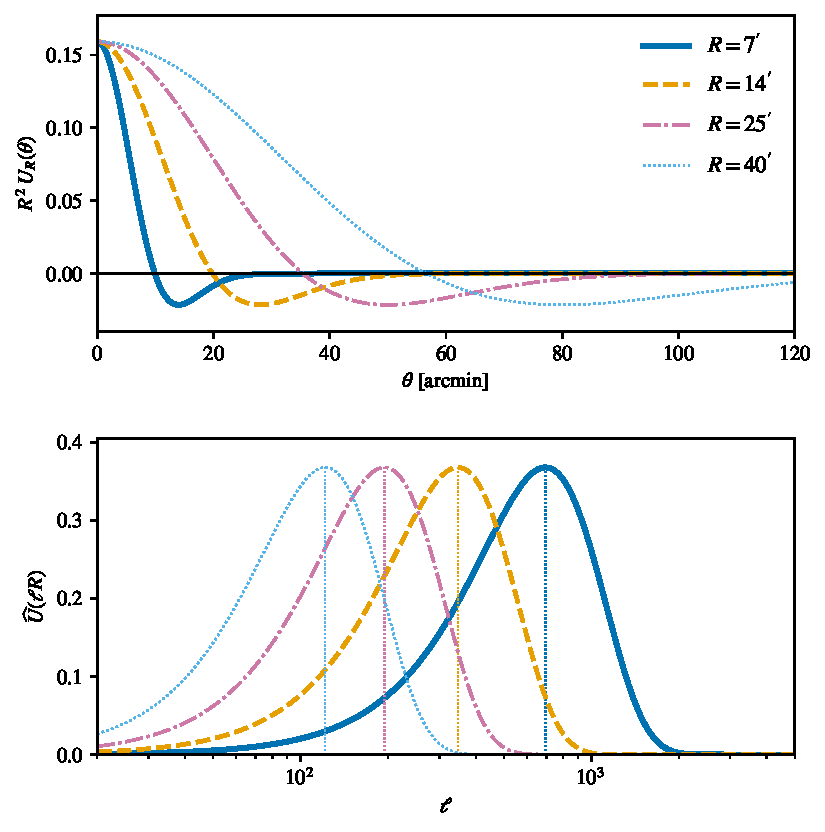
\includegraphics[width=0.62\linewidth]{plots/aperture_filter/aperture_filter.pdf}
  \caption{The compensated aperture filter at the four radii of the
    DES Y3 measurement.  Top: the real-space weight
    $\Ufil(\theta)$ of Eq.~\eqref{eq:ufil}, scaled by $R^2$ so the
    four curves share one axis.  Bottom: the Fourier window
    $\Uhat(\ell R)$ of Eq.~\eqref{eq:uhat}; each curve peaks at
    $\ell = \sqrt{2}/R$ with value $1/e$.  Drawn by the companion
    notebook (plots/aperture\us filter).}
  \label{fig:filter}
\end{figure}

\subsection{The shear form, and the E/B split}
\label{sec:qform}

\paragraph{The same number from shapes.}
Equation~\eqref{eq:mapdef} needs a convergence map, which is not what
surveys deliver; they deliver galaxy ellipticities, that is, noisy
samples of the shear.  The classical result of aperture-mass theory
is that the \emph{same} $\Map$ is obtained from the tangential shear
(Eq.~\eqref{eq:tangential}) with a different radial weight
$\Qfil$~\cite{JBJ}:
\begin{equation}
  \Map(R;\btheta_0)
  \;=\; \int d^2\theta\;
  \Qfil\bigl(|\btheta - \btheta_0|\bigr)\,
  \gamma_t(\btheta;\btheta_0),
  \qquad
  \Qfil(\theta) \;=\;
  \frac{2}{\theta^2}\int_0^{\theta} d\theta'\,\theta'\,
  \Ufil(\theta') \;-\; \Ufil(\theta) .
  \label{eq:qrelation}
\end{equation}
The relation between $\Qfil$ and $\Ufil$ follows from
Eq.~\eqref{eq:gammakappa}; the derivation (a Fourier-space exercise)
is in Schneider, Kilbinger \& Lombardi~\cite{SKL}, and the companion
notebook verifies the equality numerically on a simulated map (its
Section~3).  For the Gaussian filter~\eqref{eq:ufil} the weight is
\begin{equation}
  \Qfil(\theta)
  \;=\; \frac{\theta^2}{4\pi R^4}\;
  e^{-\theta^2/2R^2} ,
  \label{eq:qfil}
\end{equation}
the form quoted by the DES papers~\cite{GomesTATT}.  Because
$\gamma_t$ is built from measured shapes, Eq.~\eqref{eq:qrelation}
turns $\Map$ into a direct observable, no mass map needed.

\paragraph{The B-mode partner.}
Replace $\gamma_t$ by the cross component $\gamma_\times$ in
Eq.~\eqref{eq:qrelation} and the result, called $\Mx$, filters the
B~mode exactly as $\Map$ filters the E~mode.  For pure weak lensing
$\langle \Mx \rangle$-statistics built from odd powers of $\Mx$
vanish; they are the standard null test.  This clean E/B separation,
inherited from the compensated filter, is a second reason the
aperture mass is the statistic of choice: intrinsic alignments can
produce B~modes, and a statistic that keeps E and B apart can show
them (Section~\ref{sec:ia}; the separation is exact only for the
infinite filter integral, a caveat Section~\ref{sec:finite} takes
up).

\section{The second moment}
\label{sec:map2}

\paragraph{The variance of the filtered field.}
The simplest statistic of $\Map$ is its variance at one radius.
Square Eq.~\eqref{eq:mapfourier}, take the ensemble average, and use
the power-spectrum definition~\eqref{eq:powerdef}; the Dirac delta
eats one of the two $\ell$ integrals:
\begin{equation}
  \bigl\langle \Map^2(R) \bigr\rangle
  \;=\; \int \frac{d^2\ell}{(2\pi)^2}\,
  \Uhat^2(\ell R)\, P^E_\kappa(\ell)
  \;=\; \int_0^\infty \frac{d\ell\,\ell}{2\pi}\,
  \Uhat^2(\ell R)\, P^E_\kappa(\ell) ,
  \label{eq:map2}
\end{equation}
where the superscript $E$ records that only the E-mode spectrum
enters.  Because $\Uhat^2$ is a narrow bump around
$\ell = \sqrt{2}/R$, the variance is essentially the E-mode power at
that multipole: scanning $R$ scans the spectrum.  (The analogous
statistic with $\Mx$ reads the B-mode spectrum.)

\paragraph{A worked example: white noise.}
Let the convergence be pure white noise, $P^E_\kappa(\ell) = A$ with
$A$ constant.  Substituting $x = \ell R$ in Eq.~\eqref{eq:map2},
\begin{equation}
  \bigl\langle \Map^2 \bigr\rangle
  \;=\; \frac{A}{2\pi R^2}
  \int_0^\infty dx\; x\; \frac{x^4}{4}\, e^{-x^2}
  \;=\; \frac{A}{2\pi R^2}\cdot\frac{1}{4}\,
  \underbrace{\int_0^\infty dx\, x^5 e^{-x^2}}_{=\,1}
  \;=\; \frac{A}{8\pi R^2} :
  \label{eq:map2white}
\end{equation}
the remaining integral is $\Gamma(3)/2 = 1$ (substitute $u = x^2$).
The variance falls as $1/R^2$ -- a larger aperture averages more
independent patches.  The companion notebook evaluates
Eq.~\eqref{eq:map2} numerically for this spectrum and matches the
$1/(8\pi)$ coefficient (its Section~2); the same cell is the
template for evaluating Eq.~\eqref{eq:map2} with a real spectrum.

\section{The third moment}
\label{sec:map3}

\subsection{The full-filter formula}
\label{sec:fullfilter}

\paragraph{Three windows and one bispectrum.}
Now cube the Fourier form~\eqref{eq:mapfourier}, allowing a different
radius and a different source sample on each factor, and average.
The product of three fields brings three integrals
$\int d^2\ell_i/(2\pi)^2$, a factor $(2\pi)^{-6}$ in all.  The
bispectrum definition~\eqref{eq:bispecdef} supplies
$(2\pi)^2 \delta_{\rm D}(\bell_1 + \bell_2 + \bell_3)$: the delta
removes the $d^2\ell_3$ integral, forcing
$\bell_3 = -\bell_1 - \bell_2$, and its $(2\pi)^2$ cancels one of the
three, leaving $(2\pi)^{-4}$.  Write the remaining
$d^2\ell_1\, d^2\ell_2$ in polar coordinates,
$\ell_1 d\ell_1\, d\beta_1\; \ell_2 d\ell_2\, d\beta_2$; the
integrand depends on the two directions only through
$\varphi = \beta_2 - \beta_1$ (isotropy), so the overall-rotation
angle integrates to $2\pi$ and cancels one more factor, leaving
\begin{equation}
  \bigl\langle M_1 M_2 M_3 \bigr\rangle
  \;=\;
  \int \frac{\ell_1\, d\ell_1\; \ell_2\, d\ell_2\; d\varphi}
            {(2\pi)^3}\;
  B^{ijk}_\kappa\bigl(\ell_1, \ell_2,
  |\bell_1 + \bell_2|\bigr)\;
  \Uhat(\ell_1 R_1)\, \Uhat(\ell_2 R_2)\, \Uhat(\ell_3 R_3) ,
  \label{eq:map3full}
\end{equation}
with $M_a = \Map(R_a)$ of source sample on leg $a$, and
$\ell_3 = |\bell_1 + \bell_2| = (\ell_1^2 + \ell_2^2 +
2\ell_1\ell_2\cos\varphi)^{1/2}$ closing the triangle.  This is the
\emph{full-filter} aperture third moment: three band-pass windows
select a triangle of multipoles around $\sqrt{2}/R_1$,
$\sqrt{2}/R_2$, $\sqrt{2}/R_3$, and $\langle M_1 M_2 M_3\rangle$
reads the bispectrum there.  Equal radii probe roughly equilateral
triangles; unequal radii tilt the triangle, which is why the
generalized statistic carries three radius arguments~\cite{SKL}.
The DES Y3 data vector uses equal radii only
(Eq.~\eqref{eq:radii}); the unequal-radius form matters below
because the code's kernels implement it in general.

\paragraph{The projected bispectrum.}
The convergence bispectrum of three source samples follows from
Eq.~\eqref{eq:kappadef} by the same step that takes the matter power
spectrum to the convergence power spectrum -- the Limber
approximation, which ties the angular mode $\ell$ at distance $\chi$
to the transverse wavenumber $k = \ell/\chi$ and drops correlations
along the line of sight (accurate at these multipoles):
\begin{equation}
  B^{ijk}_\kappa(\ell_1,\ell_2,\ell_3)
  \;=\;
  \int d\chi\;
  \frac{W_i(\chi)\, W_j(\chi)\, W_k(\chi)}{\chi^4}\;
  B_{\rm m}\!\left(\frac{\ell_1}{\chi}, \frac{\ell_2}{\chi},
  \frac{\ell_3}{\chi};\, z(\chi)\right),
  \label{eq:limber}
\end{equation}
with the lensing window
\begin{equation}
  W_i(\chi) \;=\;
  \frac{3\Omega_{\rm m} H_0^2}{2 c^2}\,
  \frac{\chi}{a(\chi)}\, q_i(\chi) ,
  \label{eq:window}
\end{equation}
which has units of inverse length.  A quick dimensional check:
$d\chi\, W^3 \chi^{-4} B_{\rm m}$ carries
$L \cdot L^{-3} \cdot L^{-4} \cdot L^{6} = 1$, dimensionless, as a
correlation of the dimensionless $\kappa$ must be.  The three windows
appear because the same foreground structure lenses all three source
samples; with three different samples $(i,j,k)$ the statistic is
\emph{tomographic}.

\paragraph{Counting the triplets.}
$\langle M_i M_j M_k\rangle$ is symmetric under reordering its three
equal-radius legs together with their labels, so with four source
bins the independent triplets are the unordered triples with
repetition:
\begin{equation}
  \binom{4 + 3 - 1}{3} \;=\; \frac{4\cdot 5\cdot 6}{6} \;=\; 20 ,
  \label{eq:twenty}
\end{equation}
and $20$ triplets $\times$ $4$ radii $= 80$ aperture rows -- the
counts of Section~\ref{sec:fiducial}, which the companion notebook
reads back from the dataset (its Section~5).  Figure~\ref{fig:map3}
shows the predicted $\langle\Map^3\rangle(R)$ at the fiducial point
for a few representative triplets.

\begin{figure}[tbp]
  \centering
  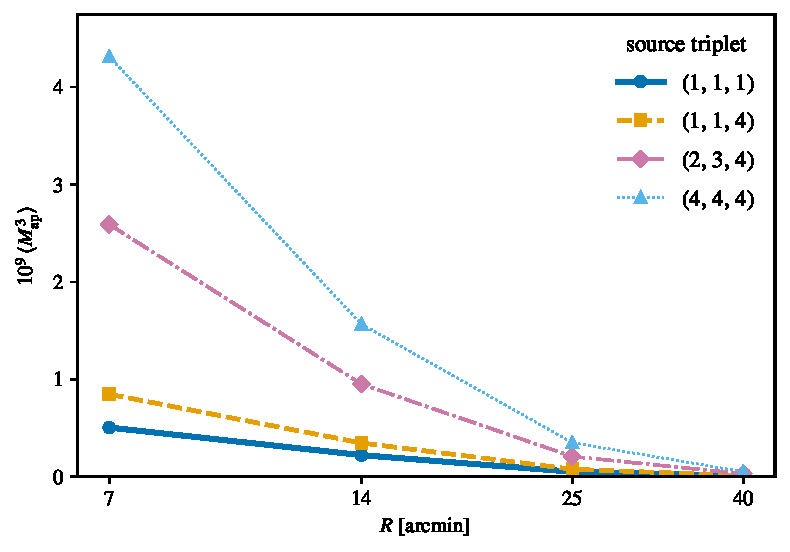
\includegraphics[width=0.62\linewidth]{plots/map3_fiducial/map3_fiducial.pdf}
  \caption{The third-order aperture-mass prediction at the fiducial
    point of Table~\ref{tab:fid}, against the filter radius $R$, for
    four of the $20$ source-bin triplets (bins numbered from 1, low
    to high redshift).  Computed through the project likelihood by
    the companion notebook (plots/map3\us fiducial); the other
    triplets interpolate between the drawn ones.}
  \label{fig:map3}
\end{figure}

\section{The real-space route: the shear three-point function}
\label{sec:threepcf}

\subsection{Why correlation functions, not maps}
\label{sec:whycorr}

Equation~\eqref{eq:map3full} is how theory thinks about
$\langle\Map^3\rangle$, but it is a poor template for a measurement:
building a convergence map and placing filter integrals on it forces
every mask, hole and ragged survey edge into the statistic, because
the filter of Eq.~\eqref{eq:ufil} extends to infinity.  Correlation
functions do not have this problem: a correlation is estimated from
pairs or triples of galaxies that both exist, so missing area removes
statistics but adds no bias~\cite{JBJ}.  The strategy of the DES
analysis -- and of this project's likelihood -- is therefore:
measure (or predict) the shear \emph{three-point correlation
function} on triangles, then integrate it with known kernels into
$\langle\Map^3\rangle$.  This section builds the two ingredients:
the natural components of the three-point function, and the kernel
integral.

\subsection{Triangles and the natural components}
\label{sec:natural}

\paragraph{Labelling a triangle.}
Three points on the sky form a triangle.  The project's grids label
it \emph{side--angle--side} (SAS): two side lengths $d_2$ and $d_3$
and the opening angle $\phi$ between them, with
$0 < \phi < \pi$.  (The excluded endpoints are degenerate, collinear
triangles, for which the projection direction used below is not
defined.)

\paragraph{The projection problem.}
A three-point average of shears, such as
$\langle \gamma(\btheta_1)\gamma(\btheta_2)\gamma(\btheta_3)\rangle$,
is not yet meaningful: each $\gamma$ carries the spin-2 phase of
Eq.~\eqref{eq:spin2}, so the raw average depends on the coordinate
axes.  The cure is to rotate each shear into a direction defined by
the triangle itself.  The project's code uses the \emph{centroid
projection}: at each vertex, the shear is rotated toward the line
from that vertex to the triangle's centroid (the mean of the three
vertices).  Write $g_a$ for the shear at vertex $a$ after this
rotation; rotating a shear toward a direction at polar angle $\beta$
means multiplying by $e^{-2i\beta}$, the spin-2 rule once more.

\paragraph{Four components, no more.}
Each of the three projected shears is complex, so products can
conjugate any subset of them.  Schneider \&
Lombardi~\cite{SchneiderLombardi} showed that exactly four
combinations transform cleanly -- a rotation of the whole triangle
multiplies each by a phase, without mixing them -- and called them
the \emph{natural components}:
\begin{equation}
  \Gamma_0 = \bigl\langle g_1 g_2 g_3 \bigr\rangle, \quad
  \Gamma_1 = \bigl\langle g_1^{*} g_2 g_3 \bigr\rangle, \quad
  \Gamma_2 = \bigl\langle g_1 g_2^{*} g_3 \bigr\rangle, \quad
  \Gamma_3 = \bigl\langle g_1 g_2 g_3^{*} \bigr\rangle ,
  \label{eq:gammas}
\end{equation}
each a complex function of the triangle $(d_2, d_3, \phi)$ and of
the ordered source-bin labels of the three vertices.  (Conjugating
two shears gives nothing new: it is the conjugate of conjugating the
third.)  The four $\Gamma_\mu$ carry the complete three-point
information of the shear field, orientation included; their relation
to the convergence bispectrum is derived in~\cite{SKL}.  Both the
complex phases and \emph{which} vertex is conjugated matter: the
same four arrays in another projection convention are different
numbers, a warning the code repeats at its interfaces.

\paragraph{How the code computes them.}
The likelihood predicts the $\Gamma_\mu$ from the bispectrum by the
multipole method of Sugiyama, Gomes \& Jarvis~\cite{fastnc},
implemented in
\texttt{cosmolike\us core/cosmolike/3pcf/transform\us 3pcf.c}.  In
outline: (i)~expand the projected bispectrum's dependence on the
triangle shape in Legendre polynomials $P_L(\mu)$, an orthogonal
polynomial basis on $[-1,1]$, where $\mu$ is defined by
$\ell_3^2 = \ell_1^2 + \ell_2^2 - 2\ell_1\ell_2\mu$;
(ii)~couple each Legendre degree $L$ to the real-space angular
harmonics $e^{iM\phi}$ through geometric coupling functions;
(iii)~turn the two Fourier side lengths into the two angular side
lengths with a pair of Bessel-function integrals, evaluated by
FFTLog (a fast Fourier transform on a logarithmic grid); and
(iv)~sum over $M$ to restore the opening angle.  The truncations
$L \le L_{\max}$ and $|M| \le M_{\max}$ are numerical settings
(Section~\ref{sec:likelihood}), to be refined like any quadrature.

\subsection{From triangles to the aperture moment}
\label{sec:sasintegral}

\paragraph{The kernel integral.}
Jarvis, Bernstein \& Jain~\cite{JBJ} (equal radii) and Schneider,
Kilbinger \& Lombardi~\cite{SKL} (general radii) carried out the
change of variables from Eq.~\eqref{eq:map3full} to real space: the
aperture third moment is an integral of the natural components over
all triangle shapes, against four closed-form complex kernels
$T_\mu$,
\begin{equation}
  \bigl\langle M_1 M_2 M_3 \bigr\rangle
  \;=\;
  {\rm Re}\,
  \frac{1}{4}\sum_{\mu=0}^{3}\;
  \int \! ds\, s \int \! \frac{d^2 t}{2\pi}\;
  \Gamma_\mu(s, \boldsymbol{t})\;
  T_\mu\!\left(\frac{s}{R_1}, \frac{\boldsymbol{t}}{R_1};
  \frac{R_2}{R_1}, \frac{R_3}{R_1}\right) ,
  \label{eq:map3sas}
\end{equation}
where the first triangle side is the real length $s = d_2$ and the
second is the complex number
$\boldsymbol{t} = d_3\, e^{i\phi}$.  The kernels are built from the
offsets $q_a$ of the three vertices from the centroid: a Gaussian
factor $e^{-Z}$ in the squared offsets (from integrating the three
Gaussian filters over the common aperture center) times polynomials
in the offsets, whose complex phases supply exactly the spin-2
rotations of the three legs; the kernel $T_\mu$ pairs with
$\Gamma_\mu$ -- conjugated leg matching conjugated leg.  Their
explicit forms are Eqs.~(62)--(69) of~\cite{SKL}, implemented
line by line in \texttt{aperture\us 3pcf.c}; this note does not
repeat them, because every property used below (which triangle sizes
contribute, how unequal radii enter) is visible in the structure
just described.  Unequal radii enter only through dimensionless
weights built from $R_2/R_1$ and $R_3/R_1$; for equal radii the
kernels reduce to the two functions $T_0$ and $T_1$
of~\cite{JBJ} (with $T_2$ and $T_3$ obtained by relabeling the
vertices).

\paragraph{The discrete sum the code evaluates.}
On the measured grid the integral becomes a sum over the SAS bins.
With logarithmic side bins of common width $\Delta\ln d$ (so
$ds = s\, d\ln d$) and linear angle bins of width $\Delta\phi$, the
measure of one triangle bin is
\begin{equation}
  \frac{s^2\, |t|^2}{2\pi}\,
  (\Delta\ln d)^2\, \Delta\phi ,
  \qquad
  s = \frac{d_2}{R_1}, \quad |t| = \frac{d_3}{R_1} ,
  \label{eq:measure}
\end{equation}
dimensionless because the sides are measured in units of $R_1$.  The
code of \texttt{aperture\us 3pcf.c} precomputes, for each radius
triplet, complex weights $W_{\mu b}$ that fold together the kernel,
this measure, the overall $1/4$, and a second kernel evaluation with
$R_2$ and $R_3$ exchanged -- the mirrored-orientation convention of
the DES Y6 aperture calculation, which accounts for each triangle's
reflection since the grid stores only $0 < \phi < \pi$.  The
aperture moment is then one dot product per radius and source
triplet,
\begin{equation}
  \bigl\langle M_1 M_2 M_3 \bigr\rangle_{\rm grid}
  \;=\;
  {\rm Re} \sum_{\mu=0}^{3} \sum_{b}
  W_{\mu b}\, \Gamma_{\mu b}
  \;=\;
  \sum_{\mu, b}
  \Bigl[\,{\rm Re}\,W_{\mu b}\, {\rm Re}\,\Gamma_{\mu b}
  \;-\; {\rm Im}\,W_{\mu b}\, {\rm Im}\,\Gamma_{\mu b}\Bigr] ,
  \label{eq:gridsum}
\end{equation}
where $b$ runs over the kept triangle bins.  There is no complex
conjugation in this product, and the factor $1/4$ is already inside
the weights.  This sum -- Eq.~\eqref{eq:gridsum} over the measured
bins -- is precisely what both the DES measurement pipeline and the
\texttt{des\us 3pcf} likelihood compute; they share the estimator by
construction.

\section{Finite triangles versus the full filter}
\label{sec:finite}

\paragraph{Two different estimators.}
Equation~\eqref{eq:map3sas} integrates over \emph{all} triangles:
sides from zero to infinity, every opening angle.
Equation~\eqref{eq:gridsum} sums over the \emph{measured} bins: in
this project, sides between $8$ and $80$ arcmin
(Section~\ref{sec:likelihood}).  These are two different statistics.
The missing triangles are not a numerical error that refinement
removes -- making the kept bins denser changes nothing about the
region that is absent.  A measurement that excludes all triangles
with a side below some cut simply measures a different (perfectly
well-defined) number than the infinite integral, and the two must
not be mixed in one analysis without quantifying their difference.
For the same reason the exact E/B separation of
Section~\ref{sec:qform} holds only for the full integral: finite
triangle coverage can mix a little of the B~pattern into the
E-selected sum, even when the underlying field is pure E.

\paragraph{Which triangles the data keep.}
Figure~\ref{fig:coverage} shows the side plane of the SAS grid: the
$20 \times 20$ logarithmic side bins of the measurement and the
$9 \times 9$ block the scale cut keeps, next to the four filter
scales.  Each kept side pair carries $63$ opening-angle bins
(Section~\ref{sec:likelihood}).  The kernels of
Eq.~\eqref{eq:map3sas} weight triangles with sides of order the
aperture radii, so for the smallest radius, $R = 7$ arcmin, much of
the kernel support sits below the $8$ arcmin cut: the finite sum
differs most from the full integral there.  Quantifying that
difference per radius is an estimator study, not a side effect of
this note.

\begin{figure}[tbp]
  \centering
  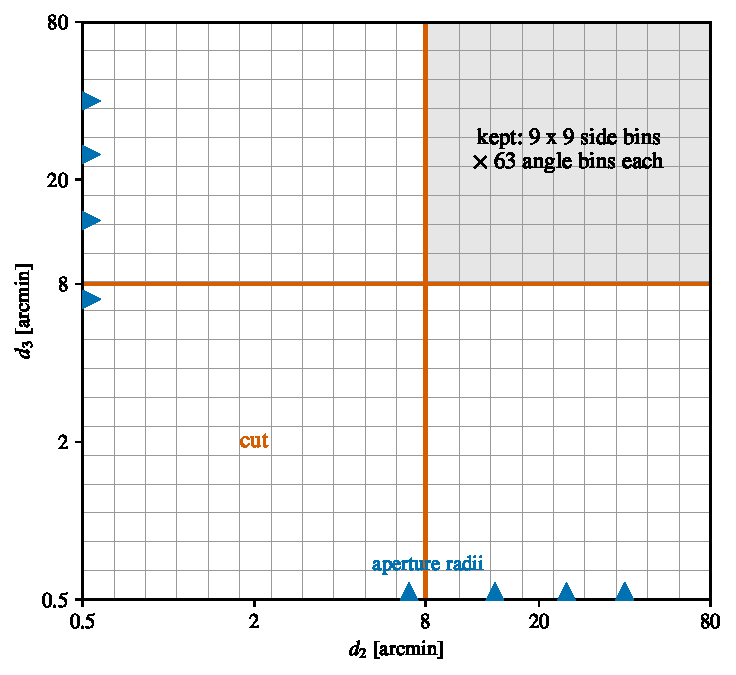
\includegraphics[width=0.62\linewidth]{plots/triangle_coverage/triangle_coverage.pdf}
  \caption{The side plane $(d_2, d_3)$ of the SAS triangle grid: the
    $20$ logarithmic side bins of the DES Y3 measurement between
    $0.5$ and $80$ arcmin, and (shaded) the $9 \times 9$ side-bin
    block kept by the $8$ arcmin lower-edge cut, every pair carrying
    $63$ opening-angle bins.  The marks on the axes are the four
    aperture radii.  Drawn by the companion notebook
    (plots/triangle\us coverage).}
  \label{fig:coverage}
\end{figure}

\paragraph{The covariance consequence.}
A likelihood needs the covariance of its data vector -- the matrix of
fluctuations of the \emph{estimator actually used}.  The compiled
analytic covariance of this project
(\texttt{cosmolike\us core/cosmolike/3pcf/COVARIANCE.md}) codes the
full-filter estimator, Eq.~\eqref{eq:map3full}; no finite-SAS
covariance has been implemented.  Because the finite-triangle Map3
is a different estimator, the project \emph{refuses} to produce
analytic Map3 covariance rows: the covariance driver requires its
\texttt{--xi-only} flag, and both the driver and the adapter state
the refusal before any numerical work
(\texttt{covariance/README.md}).  The examples read a
simulation-estimated joint covariance instead, built by measuring
the same finite-SAS estimator on synthetic maps.  The one published
test of an analytic covariance against this estimator family (Linke
et al.~\cite{Linke}, Section~5.2.2) used TreeCorr's earlier
triangle binning; none has been made against the LogMultipole
measurement behind the DES Y3 vectors.

\section{The DES Y3 measurement and the likelihood}
\label{sec:likelihood}

\subsection{What was measured}
\label{sec:measurement}

The Y3 aperture moments (Gomes et al.~\cite{GomesMethods,
GomesData}) were measured from the DES Y3 shape catalogue:
\begin{itemize}
  \item The three-point correlations were measured with TreeCorr
    5.1.1's LogMultipole method -- which accumulates the correlation
    directly in the angular harmonics $e^{iM\phi}$ of
    Section~\ref{sec:natural} -- with multipole cutoff
    $n_{\max} = 100$, that is $2 \times 100 + 1 = 201$ multipole
    values (the notebook does this arithmetic in its Section~6).
  \item The side bins are $20$ logarithmic bins from $0.5$ to $80$
    arcmin.  The result was converted from the multipole form to the
    SAS form of Section~\ref{sec:natural}.
  \item The scale cut keeps the $9$ side bins whose lower edge is at
    least $8$ arcmin.
  \item The aperture moments use the four equal radii of
    Eq.~\eqref{eq:radii} and all $20$ source-bin triplets
    (Eq.~\eqref{eq:twenty}): $80$ rows.
  \item The statistic is measured from the catalogue directly, so
    the likelihood applies no pixel window.
\end{itemize}

\subsection{What the likelihood computes}
\label{sec:likelihoodcalc}

\paragraph{The settings.}
The likelihood defaults in \texttt{likelihood/joint\us shear.yaml}
mirror the measurement:
\texttt{theta\us min\us arcmin: 0.5},
\texttt{theta\us max\us arcmin: 80},
\texttt{ntheta: 20} (the side bins),
\texttt{theta\us lower\us cut\us arcmin: 8} (the scale cut) and
\texttt{phi\us bins: 63} (the opening-angle bins).  Its
\texttt{initialize}
(\texttt{likelihood/\us cosmolike\us prototype\us base.py}) builds
the $21$ logarithmic edges from $0.5$ to $80$ arcmin, keeps the $9$
lower edges at or above $8$ arcmin, records the common logarithmic
width $\Delta\ln d = \ln(160)/20 \approx 0.2538$ (the notebook
computes it, its Section~5), places the opening-angle nodes at the
centres of $63$ equal cells of $(0, \pi)$, and constructs one fixed
transform plan (\texttt{TransformPlan.for\us aperture}) that carries
the SAS grid, the aperture kernels of Eq.~\eqref{eq:gridsum} and the
multipole machinery of Section~\ref{sec:natural}, with multipole
truncations \texttt{map\us lmax: 20} and \texttt{map\us mmax: 20}.
At every evaluation the plan turns the current bispectrum model into
the $80$ Map3 rows; the notebook wrappers expose the same numbers as
\texttt{nw.map3()}.

\paragraph{What is still open.}
Three measurement conventions are open questions: the number of
opening-angle bins used in the conversion from multipoles to SAS is
not specified in the released files; the representative side length
assigned to each logarithmic bin is not specified either; and the
theory's multipole truncation (the likelihood's
\texttt{map\us mmax: 20} against the measurement's $201$ multipole
values) has no recorded convergence target.  The project README's
estimator FAQ and
\texttt{tests/studies/estimator\us conventions.md} track them.

\section{Intrinsic alignments in the aperture moment}
\label{sec:ia}

Everything so far assumed that a galaxy's measured shape is pure
lensing.  It is not: galaxies form inside the large-scale tidal
field, and their intrinsic shapes can align with it.  This section
rebuilds, at the level of this note, the theory of that
contamination for the three-point signal -- the tidal alignment and
tidal torquing (TATT) model for the shear three-point function and
the aperture skewness of Gomes et al.~\cite{GomesTATT} -- and
connects it to the operator split the project code computes.  No
field-theory background is assumed: every ingredient is an
application of the connected-moment logic of
Section~\ref{sec:bispectrum}.

\subsection{The tidal field, and shapes that follow it}
\label{sec:tidal}

\paragraph{The tidal tensor.}
Around a forming galaxy, expand the gravitational potential $\Phi$
to second order: the gradient accelerates the galaxy as a whole, and
the matrix of second derivatives $\partial_i\partial_j\Phi$ stretches
or squeezes it along its eigendirections.  The trace of that matrix
is fixed by the local density (Poisson's equation,
$\nabla^2\Phi \propto \delta$); the shape-distorting part is the
trace-free remainder, the \emph{tidal tensor}.  Normalized by the
density field it reads, in Fourier space,
\begin{equation}
  \tilde s_{ij}(\bk)
  \;=\;
  \left(\frac{k_i k_j}{k^2} - \frac{1}{3}\delta_{ij}\right)
  \tilde\delta(\bk) ,
  \label{eq:sij}
\end{equation}
where $\delta_{ij}$ is the Kronecker delta (one for $i = j$, zero
otherwise) and the $k_ik_j/k^2$ factor is the Fourier form of
$\partial_i\partial_j/\nabla^2$.  A galaxy whose intrinsic shape
responds to the local tidal field acquires an \emph{intrinsic shear}
$\gamma_{\rm I}$: a shape correlation with the matter field that has
nothing to do with light deflection.

\paragraph{The observed shape is a sum.}
At the level of the shear, the measured quantity is
\begin{equation}
  \gamma \;=\; \gamma_{\rm G} + \gamma_{\rm I} ,
  \label{eq:gsum}
\end{equation}
lensing plus intrinsic.  (Shape estimators respond to ellipticity,
not shear, by a responsivity factor; the model absorbs that factor
into the alignment amplitudes~\cite{GomesTATT}.)  The key
difference between the two terms is \emph{where} they live: the
lensing part of a source in bin $a$ integrates all foreground matter
with the kernel $W_a$ of Eq.~\eqref{eq:window}, while the intrinsic
part is generated at the galaxy's own distance, weighted by the
source distribution itself.

\paragraph{Eight placements.}
Insert Eq.~\eqref{eq:gsum} into a three-point average and expand --
plain algebra, the same as expanding $(G + I)^3$ while keeping track
of which factor sits on which leg:
\begin{equation}
  \bigl\langle \gamma^a \gamma^b \gamma^c \bigr\rangle
  = \langle G G G\rangle
  + \bigl[\langle I G G\rangle + \langle G I G\rangle
        + \langle G G I\rangle\bigr]
  + \bigl[\langle I I G\rangle + \langle I G I\rangle
        + \langle G I I\rangle\bigr]
  + \langle I I I\rangle ,
  \label{eq:placements}
\end{equation}
eight terms: the pure lensing signal and seven contamination
pieces.  With unequal source bins the three placements inside each
bracket are genuinely different numbers -- an intrinsic shape in the
low-redshift bin correlates with the lensing of the bins behind it,
but not the reverse -- which is why the code tracks \emph{ordered}
legs.  These eight \emph{placements},
labelled GGG, GGI, GIG, IGG, GII, IGI, IIG, III, are one axis of the
project's diagnostic split; the physical \emph{operators} below are
the other.

\subsection{NLA: the linear response}
\label{sec:nla}

\paragraph{One coefficient, one kernel trick.}
The simplest model takes the intrinsic shear linear in the tidal
field (tidal alignment), with the nonlinear matter field inserted --
the \emph{nonlinear linear alignment} model, NLA~\cite{HirataSeljak,
BridleKing}.  Its coefficient carries an amplitude $A_1$ and a
redshift power law,
\begin{equation}
  f_{\rm IA}(z)
  \;=\;
  -\,A_1
  \left(\frac{1+z}{1+z_0}\right)^{\eta_1}
  \frac{\bar C_1\, \rho_{\rm crit}\, \Omega_{\rm m}}{D(z)} ,
  \label{eq:fia}
\end{equation}
with $z_0 = 0.62$ the pivot redshift of the DES convention (at
$z = z_0$ the bracket is one), $D(z)$ the linear growth factor,
$\rho_{\rm crit}$ the critical density, and $\bar C_1$ a fixed
normalization constant; CosmoLike's native normalization and pivot
are used throughout the project, and the companion notebook prints
the alignment record the likelihood actually uses (its Section~7).
Because this intrinsic shear is proportional to the same matter
field that sources the lensing, every statistic of
Section~\ref{sec:map3} absorbs NLA by one replacement in the lensing
efficiency~\cite{GomesTATT}:
\begin{equation}
  q_a(\chi)
  \;\longrightarrow\;
  q_a(\chi) + f_{\rm IA}\bigl(z(\chi)\bigr)\,
  p_a(\chi)\, \frac{dz}{d\chi} ,
  \label{eq:nlakernel}
\end{equation}
the Jacobian $dz/d\chi$ converting the redshift-space source density
into a density per distance.  Nothing else changes: the bispectrum
model is untouched, and all eight placements of
Eq.~\eqref{eq:placements} are generated at once by the modified
kernels.  That economy is NLA's appeal -- and its limit, because a
linear response cannot describe shapes built by \emph{tidal
torquing}, the spin acquired by rotation-supported galaxies, which
is quadratic in the tidal field.

\subsection{TATT: the expansion to second order}
\label{sec:tatt}

\paragraph{The model.}
TATT~\cite{Blazek} expands the three-dimensional intrinsic shape
tensor in powers of the tidal field, keeping every term to second
order:
\begin{equation}
  \gamma^{\rm I}_{ij}
  \;=\;
  C_1\, s_{ij}
  \;+\;
  C_{1\delta}\, \bigl(\delta\, s_{ij}\bigr)
  \;+\;
  C_2 \left(s_{ik} s_{kj}
  - \frac{1}{3}\delta_{ij}\, s^2\right) ,
  \label{eq:tattdef}
\end{equation}
with repeated indices summed and $s^2 = s_{kl}s_{kl}$.  Each term is
readable in plain words:
\begin{itemize}
  \item $C_1 s_{ij}$: the linear tidal alignment of
    Section~\ref{sec:nla}; $C_1$ is identified with
    $f_{\rm IA}$ of Eq.~\eqref{eq:fia}.
  \item $C_{1\delta}\,\delta s_{ij}$: \emph{density weighting}.
    Shapes are only observed where galaxies sit, and galaxies sit
    preferentially in overdense regions; sampling the alignment at
    galaxy positions multiplies it by the local density.  The DES
    convention ties its coefficient to the linear one through a bias
    parameter, $C_{1\delta} = b_{\rm TA} C_1$.
  \item $C_2 (s s - {\rm tr}/3)$: \emph{tidal torquing}, quadratic
    in the tidal field, with its own amplitude and redshift law,
    \begin{equation}
      C_2 \;=\; 5 A_2
      \left(\frac{1+z}{1+z_0}\right)^{\eta_2}
      \frac{\bar C_1\, \rho_{\rm crit}\, \Omega_{\rm m}}{D^2(z)} .
      \label{eq:c2law}
    \end{equation}
\end{itemize}
The parameter set $(A_1, \eta_1, A_2, \eta_2, b_{\rm TA})$ is the
one the project yamls sample; at the TATT point of
Eq.~\eqref{eq:tattpoint} all three operators are active.  The
observable intrinsic shear is the projection of
Eq.~\eqref{eq:tattdef} onto the sky plane, which turns the symmetric
trace-free $3\times 3$ tensor into the complex spin-2 combination of
Eq.~\eqref{eq:gammacomplex}, split into its E and B parts.

\paragraph{Why quadratic terms matter for a third moment.}
Here the connected-moment logic of Section~\ref{sec:bispectrum} pays
off.  Treat the linear density field as Gaussian.  A three-point
average of three \emph{linear} quantities then vanishes
(Section~\ref{sec:bispectrum}): the NLA contamination of the
bispectrum exists only because the matter bispectrum itself is
non-Gaussian.  But a \emph{quadratic} term is a new source: one
second-order factor and two linear factors give, exactly as in
Eq.~\eqref{eq:treeidea}, a nonvanishing Gaussian average
proportional to two power spectra.  Every second-order operator of
Eq.~\eqref{eq:tattdef} -- density weighting, tidal torquing, and the
second-order part of gravity itself -- therefore contributes to the
three-point signal at the lowest (``tree'') order with the universal
structure
\begin{equation}
  B(\bk_1,\bk_2,\bk_3)
  \;=\;
  2\, K^{(1)}(\bk_1)\, K^{(1)}(\bk_2)\,
  K^{(2)}(\bk_1,\bk_2)\;
  P_{\rm L}(k_1)\, P_{\rm L}(k_2)
  \;+\; \text{2 permutations},
  \label{eq:treegeneral}
\end{equation}
where $K^{(1)}$ and $K^{(2)}$ are the first- and second-order
response kernels of whichever pair of fields sits on the legs
(density or shape), and the permutations move the second-order
kernel to the other two legs~\cite{GomesTATT}.  For three density
legs with the gravity kernels this is exactly
Eq.~\eqref{eq:btree}; for shape legs the kernels follow from
Eq.~\eqref{eq:tattdef} and the projection onto E and B.

\paragraph{The E-mode bispectra.}
Projecting each leg onto density ($\delta$), E or B gives the
intrinsic-alignment bispectra.  Gomes et al.\ derive them by
specializing the general effective-field-theory shape kernels (their
Section II) to the TATT coefficients; the dictionary is
$c^g_1 = 2C_1$, $c^g_{2,2} = C_2$ and
$c^g_{2,3} = C_{1\delta} - \tfrac{2}{3} C_2$~\cite{GomesTATT}.
The simplest output, written with the third wavevector along the
$x$ axis and hats denoting unit-vector components, is the
density--density--E bispectrum,
\begin{equation}
\begin{split}
  B_{\delta\delta E}(\bk_1,\bk_2,\bk_3)
  \;=\;& C_1\, B^{\rm tree}_{\delta}(\bk_1,\bk_2,\bk_3) \\
  &+ C_2\, P_{\rm L}(k_1) P_{\rm L}(k_2)
  \Bigl(\tfrac{1}{2}(\hat\bk_1\!\cdot\!\hat\bk_2)
  (\hat k_{1x}\hat k_{2x} - \hat k_{1y}\hat k_{2y}) \\
  &\hspace{8.2em}
  - \tfrac{1}{12}(\hat k_{1x}^2 - \hat k_{1y}^2
  + \hat k_{2x}^2 - \hat k_{2y}^2)\Bigr) \\
  &+ C_{1\delta}\, P_{\rm L}(k_1) P_{\rm L}(k_2)
  \left(\tfrac{1}{2}(\hat k_{1x}^2 - \hat k_{1y}^2
  + \hat k_{2x}^2 - \hat k_{2y}^2)\right) ,
\end{split}
  \label{eq:bdde}
\end{equation}
with $B^{\rm tree}_\delta$ from Eq.~\eqref{eq:btree}.  Each line is
one operator: the $C_1$ line is the linear response riding on the
matter bispectrum; the $C_2$ and $C_{1\delta}$ lines are the new
tree-level terms of Eq.~\eqref{eq:treegeneral}, their unit-vector
polynomials being the spin-2 projections of the quadratic kernels.
The bispectra with two and three shape legs, $B_{\delta EE}$ and
$B_{EEE}$, have the same structure with coefficients
$C_1 C_2$, $C_1 C_{1\delta}$, $C_1^2 C_2$, $C_1^2 C_{1\delta}$ and
longer (but still closed-form) shape polynomials, written
in~\cite{GomesTATT} through auxiliary functions $U, V, W, T$ of the
triangle; this note does not transcribe them.  Two structural facts
matter here.  First, every higher-placement term carries extra
powers of $C_1$: a quadratic operator on one leg needs linear
responses on the other shape legs.  Second, at tree level the only
nonvanishing B-mode bispectra have exactly \emph{one} B leg
(for example $B_{\delta\delta B} \propto C_2 + 3C_{1\delta}$).  The
reason is geometric.  Projecting a symmetric tensor onto E and B
along a wave direction works like polarization: the E part is the
stretch aligned with or perpendicular to the wavevector (a
$\cos 2\phi_k$ pattern around it), the B part the stretch at
$45^\circ$ (a $\sin 2\phi_k$ pattern).  The first-order shape kernel
is $\tilde s_{ij}$ of Eq.~\eqref{eq:sij}, which stretches exactly
along its own wavevector -- pure E, no B part.  A B leg therefore
needs a \emph{second-order} kernel on it, and each tree-level term
of Eq.~\eqref{eq:treegeneral} has only one second-order kernel to
spend, so at most one leg can be~B.  On nonlinear scales the model
follows the NLA
phenomenology: $P_{\rm L}$ is replaced by the nonlinear spectrum,
and the $C_1\,B^{\rm tree}_\delta$ pieces by the BiHalofit
bispectrum~\cite{GomesTATT}.

\subsection{Projection, and the eight-term aperture moment}
\label{sec:iaprojection}

\paragraph{Two kernels per line of sight.}
Each three-dimensional bispectrum is projected onto the sky exactly
as in Eq.~\eqref{eq:limber}, with one difference per leg: a lensing
(G) leg of source bin $a$ keeps the lensing window
$W_a$ of Eq.~\eqref{eq:window}, while an intrinsic (I) leg selects
the source population at the local distance, with the window
$W_{g,a} \propto p_a(\chi)$ -- the same replacement logic as
Eq.~\eqref{eq:nlakernel}, now applied leg by leg.  Summing every
placement of Eq.~\eqref{eq:placements} gives the total aperture
moment as eight projected terms~\cite{GomesTATT}: schematically,
\begin{equation}
  \bigl\langle M^3 \bigr\rangle^{ijk}_{\rm total}
  \;=\;
  \int d\chi \sum_{\rm placements}
  \frac{W^{i}_{(\cdot)} W^{j}_{(\cdot)} W^{k}_{(\cdot)}}{\chi^4}\;
  \bigl\langle M^3\bigr\rangle_{(\cdot)}\bigl(z(\chi)\bigr) ,
  \label{eq:map3total}
\end{equation}
where each placement picks $W_\kappa$ or $W_g$ per leg and the
matching bispectrum component ($\delta$ or E on that leg).  In the
DES implementation the first term -- all lensing, plus the linear
alignment absorbed into the kernels by
Eq.~\eqref{eq:nlakernel} -- rides on the full BiHalofit bispectrum,
and the seven others carry the higher-order TATT pieces.

\paragraph{The code's operator split.}
The project's diagnostic call,
\texttt{nw.map3\us components()}, computes each Map3 row as a
$5 \times 8$ table: five physical \emph{operators} -- gravity-only
lensing, linear alignment, density weighting, tidal torquing, and
the optional velocity shear below -- by the eight \emph{placements}
of Eq.~\eqref{eq:placements}, with the sum checked against the
ordinary total.  The split follows the coefficient structure above;
one subtlety, inherited from the kernel dictionary, is that a
torque-only selection must keep both the $C_2$ kernel and the
$-\tfrac{2}{3}C_2$ piece of the density-shaped vertex, while a
density-weighting selection keeps only $C_{1\delta}$
(\texttt{cosmolike\us core/cosmolike/3pcf/README.md}).
Figure~\ref{fig:operators} shows the split at the TATT point of
Eq.~\eqref{eq:tattpoint} for one low-redshift triplet, where the
alignment terms are largest; the companion notebook computes it
through the project likelihood (its Section~7).  At this point the
linear alignment adds between $+8.5$ and $+11$ percent to the
gravity-only rows of the lowest-redshift triplet (the fiducial
$A_1 = -0.33$ raises the signal, because the alignment coefficient
of Eq.~\eqref{eq:fia} carries a minus sign), while the
density-weighting term stays below $0.2$ percent in magnitude and
the tidal-torquing term below $0.7$ percent, changing sign at the
largest radius; the notebook also checks that the $5 \times 8$
pieces add back to the ordinary prediction to machine precision.

\begin{figure}[tbp]
  \centering
  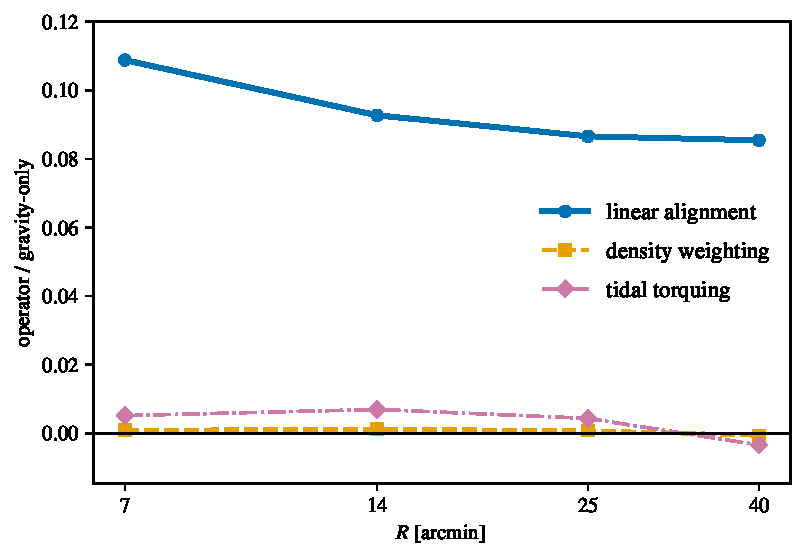
\includegraphics[width=0.62\linewidth]{plots/map3_operators/map3_operators.pdf}
  \caption{The intrinsic-alignment operator split of the aperture
    moment at the TATT point (Eq.~\eqref{eq:tattpoint}), for the
    lowest-redshift source triplet: each curve is one physical
    operator's contribution, summed over its galaxy placements and
    divided by the gravity-only term, against the filter radius.
    The velocity-shear amplitude is zero, as in the likelihood.
    Computed by the companion notebook
    (plots/map3\us operators).}
  \label{fig:operators}
\end{figure}

\subsection{What the quadratic terms do, and what remains open}
\label{sec:iaresults}

\paragraph{The headline findings of the TATT paper.}
Three results of Gomes et al.~\cite{GomesTATT} shape how this
project uses the model.  First, the TATT contamination varies much
more strongly across triangle shapes than NLA's, with the skewed
(elongated) configurations most affected -- a shape dependence the
unit-vector polynomials of Eq.~\eqref{eq:bdde} make plausible.
Second, for alignment parameters of order unity the NLA and TATT
predictions of the aperture skewness differ at about the ten percent
level.  Third, the higher-order terms can push the two- and
three-point signals in \emph{opposite} directions -- damping
$\xi_\pm$ while boosting $\langle\Map^3\rangle$ -- so a joint
analysis can break the degeneracy between alignment amplitude and
fluctuation amplitude that either statistic alone leaves open.  The
Fisher companion of this project's intrinsic-alignment note
(\texttt{notes/intrinsic\us alignments}) quantifies that
degeneracy-breaking for the DES Y3 setup; this note stops at the
theory.

\paragraph{Velocity shear.}
TATT complete at second order needs one more operator: the
\emph{velocity shear}, $C_t\, t_{ij}$, with
$t_{ij}$ the trace-free shear of the velocity field (it measures how
the velocity of matter, not its density, is being sheared; for
growing structure in linear theory $t_{ij}$ reduces to $s_{ij}$ and
the operator is degenerate with tidal alignment, so only its
nonlinear part is new).  The project implements the vertex the
upstream code evaluates, which in the equilateral limit gives
$B^{\rm VS}_{\delta\delta E} = -3 C_t P^2/14$; the corresponding
printed equations of~\cite{GomesTATT} differ from this result, and
the convention difference between manuscript and code is recorded as
unresolved
(\texttt{cosmolike\us core/cosmolike/3pcf/README.md}).  The
likelihood itself always runs with $C_t = 0$; the diagnostic wrapper
accepts a nonzero value for studies.

\paragraph{B modes and the finite grid.}
The aperture moment keeps only E modes by construction
(Section~\ref{sec:qform}) -- for the infinite filter integral.  The
tree-level TATT model does produce single-B bispectra
(Section~\ref{sec:tatt}), and the finite-SAS sum of
Section~\ref{sec:finite} does not separate E from B exactly, so some
leakage of the omitted single-B terms into the predicted rows is
possible in principle.  Its size has not been quantified; the core
README records this as an open control.

\section{Limits and pointers}
\label{sec:limits}

What this note does not cover, and where it lives instead:
\begin{itemize}
  \item The constraining power of the $80$ rows -- Fisher forecasts,
    the role of the joint covariance with $\xi_\pm$, NLA against
    TATT -- is the subject of the intrinsic-alignment note,
    \texttt{notes/intrinsic\us alignments}, and its notebook.
  \item The simulation covariance that the examples read (synthetic
    DES-footprint maps, TreeCorr measurement of the same finite-SAS
    estimator) is derived in \texttt{notes/gptg\us simulations} and
    \texttt{notes/covariance\us from\us simulations}.
  \item Baryonic feedback on the bispectrum (BiHalofit responses,
    BACCO) is derived in \texttt{notes/baryonic\us feedback}.
  \item The estimator conventions still open with the measurement's
    author are tracked in
    \texttt{tests/studies/estimator\us conventions.md}.
  \item The accuracy settings of the transform (multipole caps, FFT
    grids, interpolation) are documented in the core reference,
    \texttt{cosmolike\us core/cosmolike/3pcf/README.md}, section
    ``Accuracy controls''.
\end{itemize}

\paragraph{Acknowledgements.}
\textbf{We thank Sunao Sugiyama and Rafael C. H. Gomes for their
scientific work and codes, the foundation of this project's
three-point port.}  The source projects are
\href{https://github.com/git-sunao/fastnc}{fastnc},
\href{https://github.com/rchgomes/3pcf_integrator}{3pcf\us
integrator} and
\href{https://github.com/rchgomes/desy6-3pcf}{desy6-3pcf}; the
aperture kernels follow Jarvis, Bernstein \& Jain~\cite{JBJ} and
Schneider, Kilbinger \& Lombardi~\cite{SKL}, with TreeCorr's
centroid/SAS convention by Mike Jarvis.

\begin{thebibliography}{99}

\bibitem{SchneiderLombardi}
P. Schneider and M. Lombardi,
\emph{The three-point correlation function of cosmic shear: I. The
natural components},
A\&A 397 (2003) 809,
\href{https://arxiv.org/abs/astro-ph/0207454}{arXiv:astro-ph/0207454}.

\bibitem{SKL}
P. Schneider, M. Kilbinger and M. Lombardi,
\emph{The three-point correlation function of cosmic shear: II.
Relation to the bispectrum of the projected mass density and
generalized third-order aperture measures},
A\&A 431 (2005) 9,
\href{https://arxiv.org/abs/astro-ph/0308328}{arXiv:astro-ph/0308328}.

\bibitem{JBJ}
M. Jarvis, G. Bernstein and B. Jain,
\emph{The skewness of the aperture mass statistic},
MNRAS 352 (2004) 338,
\href{https://arxiv.org/abs/astro-ph/0307393}{arXiv:astro-ph/0307393}.

\bibitem{Crittenden}
R. G. Crittenden, P. Natarajan, U.-L. Pen and T. Theuns,
\emph{Discriminating weak lensing from intrinsic spin correlations
using the curl-gradient decomposition},
ApJ 568 (2002) 20,
\href{https://arxiv.org/abs/astro-ph/0012336}{arXiv:astro-ph/0012336}.

\bibitem{fastnc}
S. Sugiyama, R. C. H. Gomes and M. Jarvis,
\emph{Fast modeling of the shear three-point correlation function},
\href{https://arxiv.org/abs/2407.01798}{arXiv:2407.01798}.

\bibitem{GomesMethods}
R. C. H. Gomes et al.,
\emph{Cosmology with second and third-order shear statistics for the
Dark Energy Survey: Methods and simulated analysis},
\href{https://arxiv.org/abs/2503.03964}{arXiv:2503.03964}.

\bibitem{GomesData}
R. C. H. Gomes et al.,
\emph{Dark Energy Survey Year 3: Cosmological constraints from
second and third-order shear statistics},
\href{https://arxiv.org/abs/2508.14018}{arXiv:2508.14018}.

\bibitem{GomesTATT}
R. C. H. Gomes et al.,
\emph{Tidal alignment and tidal torquing modeling for the cosmic
shear three-point correlation function and mass aperture skewness},
\href{https://arxiv.org/abs/2601.09133}{arXiv:2601.09133}.

\bibitem{Blazek}
J. Blazek, N. MacCrann, M. A. Troxel and X. Fang,
\emph{Beyond linear galaxy alignments},
Phys. Rev. D 100 (2019) 103506,
\href{https://arxiv.org/abs/1708.09247}{arXiv:1708.09247}.

\bibitem{HirataSeljak}
C. M. Hirata and U. Seljak,
\emph{Intrinsic alignment-lensing interference as a contaminant of
cosmic shear},
Phys. Rev. D 70 (2004) 063526,
\href{https://arxiv.org/abs/astro-ph/0406275}{arXiv:astro-ph/0406275}.

\bibitem{BridleKing}
S. Bridle and L. King,
\emph{Dark energy constraints from cosmic shear power spectra:
impact of intrinsic alignments on photometric redshift
requirements},
New J. Phys. 9 (2007) 444,
\href{https://arxiv.org/abs/0705.0166}{arXiv:0705.0166}.

\bibitem{BiHalofit}
R. Takahashi, T. Nishimichi, T. Namikawa, A. Taruya, I. Kayo,
K. Osato, Y. Kobayashi and M. Shirasaki,
\emph{Fitting the nonlinear matter bispectrum by the Halofit
approach},
ApJ 895 (2020) 113,
\href{https://arxiv.org/abs/1911.07886}{arXiv:1911.07886}.

\bibitem{Linke}
L. Linke, S. Heydenreich, P. A. Burger and P. Schneider,
\emph{A roadmap to cosmological parameter analysis with third-order
shear statistics II: Analytic covariance estimate},
A\&A (2023),
\href{https://arxiv.org/abs/2212.04485}{arXiv:2212.04485}.

\end{thebibliography}
\end{document}
